%%%%%%%%%%%%%%%%%%%%%%%%%%%%%%%%%%%%%%%%%%%%%%%%%%%%%%%%%%%%%%%%%%%%%%%%%%%%%%%%
%                   DESCRIPTION OF THE DATASETS                                %
%%%%%%%%%%%%%%%%%%%%%%%%%%%%%%%%%%%%%%%%%%%%%%%%%%%%%%%%%%%%%%%%%%%%%%%%%%%%%%%%
We present in this section the different datasets of \gls{sca} traces which will be used for the experimental validation of our work in this thesis.
Those datasets cover a large spectrum of use cases.
Moreover, most of them are publicly available, which is of great interest for -- fair -- comparison with the state of the art.
Some of those datasets are used in several parts and contributions in this thesis.
That is why, for conciseness, we gather their description in a devoted section.

\subsection{Chip Whisperer Dataset (CW)}
\label{sec:dataset_cw}
This dataset has been used in the work we presented at \textsc{Ches} 2020~\cite{masure_comprehensive_2019}.
Although it does not depict the execution of a whole cryptographic primitive, it emulates the behavior of leakages of any secret-sharing scheme that may occur during the execution of assembly instructions in a software implementation.

\paragraph{The Target.}
The leakage traces represent the power consumption of a \textsf{XMEGA128D4} chip supported on a \textsf{Chip Whisperer Lite} board~\cite{oflynn_chip_2014}.
The firmware is directly written in assembly code.
A pseudo-code is provided in \autoref{alg:assembly}.
It consists in iteratively loading a byte of a \(16\)-byte plaintext array to a register of the \gls{mcu} in order to provoke a physical leakage, then setting the value of the byte to zero and then storing it back in \gls{ram}.
The operations are then repeated for each byte of the array.

\begin{algorithm}[ht]
    \caption{\textsf{loadData}}\label{alg:assembly}
    \begin{algorithmic}[1]
        \State LD   r0, X   \Comment{Loads the first byte in r0}
        \State CLR  r0      \Comment{Clears the register}
        \State ST   X, r0   \Comment{Stores 0 in the plaintext array}

        \State LD   r0, X   \Comment{Do it again to clear the bus}
        \State CLR  r0
        \State ST   X, r0

        \State LD   r0, X   \Comment{One more time to be sure}
        \State CLR  r0
        \State ST   X+, r0
    \end{algorithmic}
\end{algorithm}
\(500,000\) traces of \(2,500\) time samples each have been acquired, along with the corresponding bytes array denoted by \verb+plain[i]+, \(i \in \llbracket 0, 15 \rrbracket\). 
The complete acquisition has been done within \(15\) hours. 

\paragraph{Quick Analysis of the Traces.}
Since this dataset will mainly be used to investigate \gls{dl}-\gls{sca} in presence of secret-sharing, we would like to prevent any leakage jointly involving two bytes of the array.
\autoref{fig:cw_trace} shows an example of one trace acquired through the platform.
The 16 patterns denoting the execution of \autoref{alg:assembly} on each byte of the array are clearly distinguishable.
We provide the corresponding \gls{snr} in \autoref{fig:snr_cw} (top) in different colors for each byte.
In addition, we have also computed a \gls{snr} of order 2, that is, targeting the \verb+xor+ between two bytes, for any couple of bytes.
The absence of peaks tends to confirm that there is no undesirable leakage, at least involving such a \verb+xor+.
However, a leakage between two bytes involving another relationship than a \verb+xor+ might still be informative, this does not allow to draw a sharp conclusion.
Emphasizing such a leakage would require many more traces to reach a significant conclusion.
That is why we let open this eventuality, although we remain confident that it is not likely to happen.
\begin{figure}[ht]
    \centering
    \begin{subfigure}{\textwidth}
        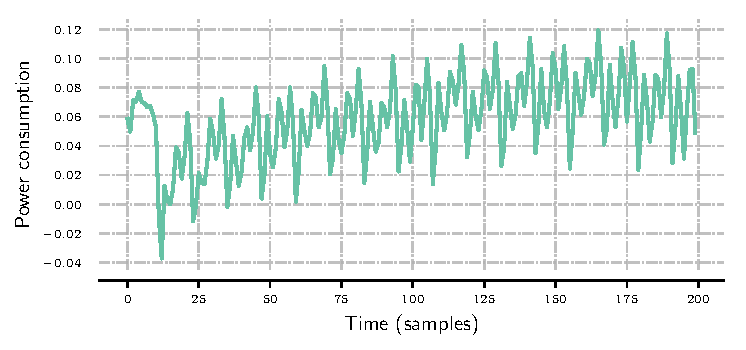
\includegraphics[width=\textwidth]{CW-dataset/exp_trace}
        \caption{Illustration of one trace}
        \label{fig:cw_trace}
    \end{subfigure}
    \begin{subfigure}{\textwidth}
        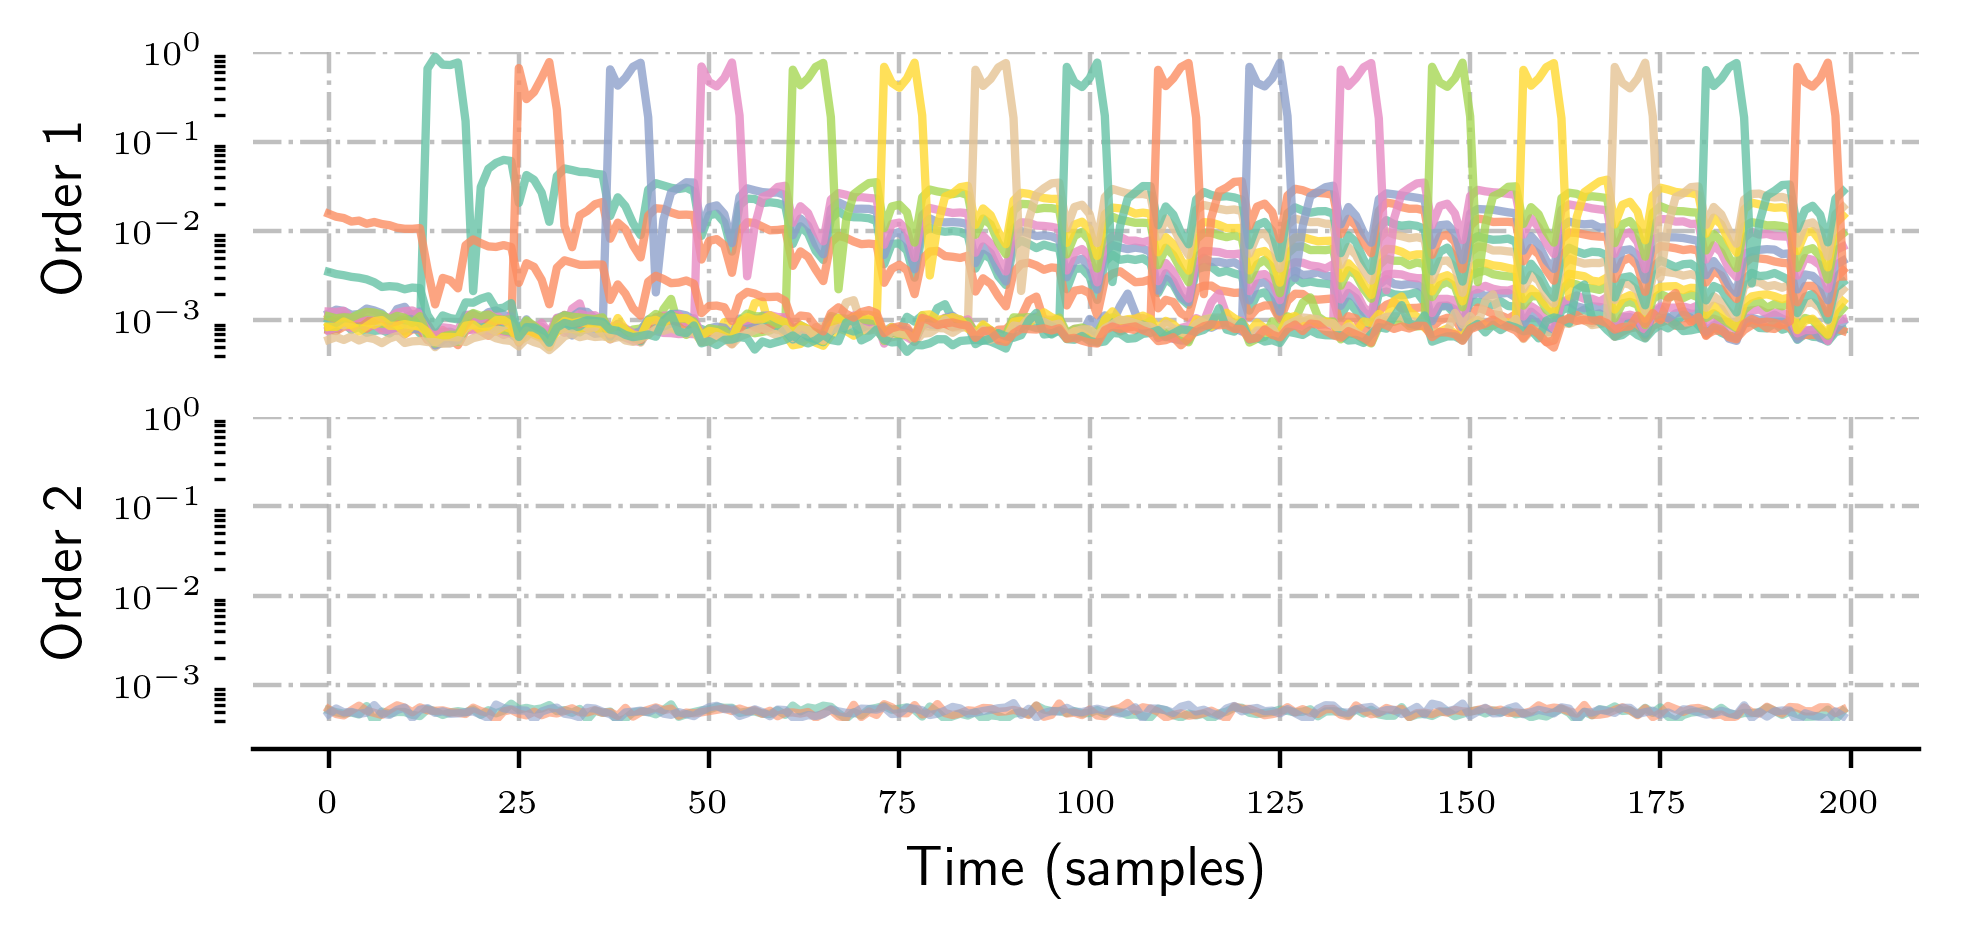
\includegraphics[width=\textwidth]{CW-dataset/snr_reduce.png}
        \caption{The \glspl{snr} of order 1 and 2 (in log scale).}
    \end{subfigure}
    \caption{The CW dataset.}
    \label{fig:snr_cw}
\end{figure}

\subsection{The ASCAD Dataset}
\label{sec:ascad}
The \gls{ascad} dataset has been introduced in 2018 by Benadjila \etal{}~\cite{prouff_study_2018} to provide the \gls{sca} community a benchmark to investigate and compare \gls{dl}-based attacks.
In particular, the aim is to assess to what extent deep learning is relevant to mount attacks against protected implementations.

\paragraph{The Target.}
The target is a protected software \gls{aes}-128 implementation running over an \textsf{ATMEGA-8515}, which has an 8-bit \textsf{AVR} architecture.
The software aims at protecting against first-order \gls{sca}, by using a Boolean secret-sharing scheme based on the table re-computation method (\cf{} \autoref{algo:table_recomputation}), although the first two bytes of the \gls{aes} state are not protected, for the sake of comparison.
Typically, the targeted variable on this dataset is the third byte of the state, at the output of the \(\Sbox\) in the first round, \ie{}, \(\Z = \fonction{\Sbox}{\p[3] \oplus \key[3]}\).
The dataset provides \(60, 000\) traces, where \(\numTracesProf = 50, 000\) traces are used for profiling and \(\numTracesVal = 10, 000\) for validation, \ie{}, for emulating attacks phases -- see \autoref{sec:estimate_practice}.
For both datasets, the same fixed key has been used, while the plaintexts and the shares have been randomly drawn.%
\footnote{
    Since the first release, a new version of the traces has been published, using a random key in the profiling traces, which are besides twice larger.
    This version is not investigated in this thesis.
}
Whereas the whole traces, focused on the first \gls{aes} round are made of \(100,000\) time samples, this thesis will focus on the chunk corresponding to the interval \(\llbracket 45,400; 46,100\rrbracket\), \ie{}, \(\traceLength = 700\).
This window corresponds to the joint leakage of \(\Z \oplus \rout\) and \(\rout\).
Three versions of this dataset are available: the first one provides the traces as is, whereas the second and third ones provide the same traces on which an artificial shift of maximum amplitude of respectively 50 and 100 points has been applied.
The traces are publicly available at \url{https://github.com/ANSSI-FR/ASCAD}.

\paragraph{Quick Analysis of the Traces.}
A characterization with the statistical methods presented in \autoref{sec:PoIs} is provided in \autoref{fig:charac_ascad}.
\autoref{fig:charac_ascad_t_test} depicts the characterization thanks to a T-test, while \autoref{fig:charac_ascad_snr} depicts the characterization done with a \gls{snr}.
\begin{figure}
    \centering
    \begin{subfigure}{0.49 \textwidth}
        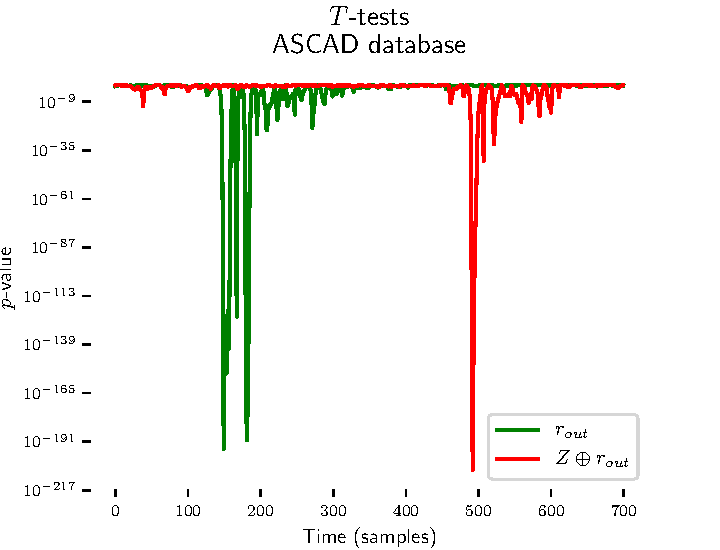
\includegraphics[width=\textwidth]{ASCAD/ttest_m_and_zxm}
        \caption{T-test}
        \label{fig:charac_ascad_t_test}
    \end{subfigure}
    \begin{subfigure}{0.49 \textwidth}
        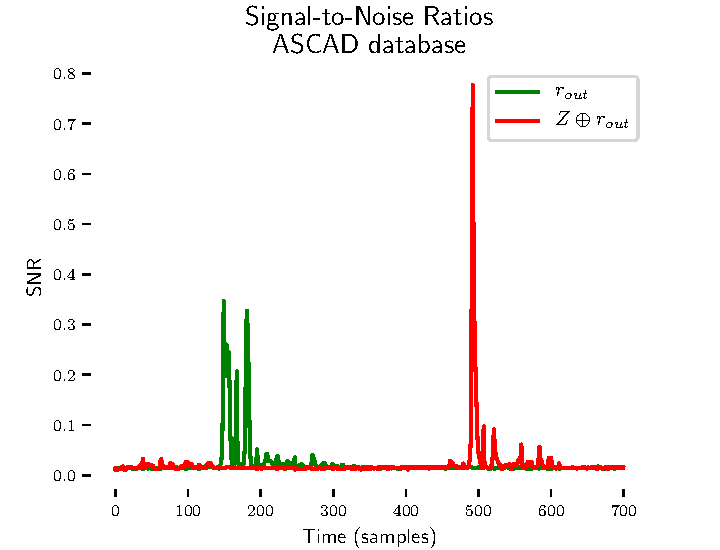
\includegraphics[width=\textwidth]{ASCAD/snr_m_and_zxm}
        \caption{\gls{snr}}
        \label{fig:charac_ascad_snr}
    \end{subfigure}
    \caption{Leakage characterization with statistical tools over the \gls{ascad} dataset, without artificial shift.}
    \label{fig:charac_ascad}
\end{figure}
On those two plots, the green peaks emphasize the leakage of the random share \(\rout\), while the red peaks denote the leakage of the output of the re-computed \(\Sbox\), namely \(\Z \oplus \rout\).
The recombination of the two leakages would give access to information about the sensitive variable \(\Z\), which might be a privileged target for an attacker.

Nevertheless the latter characterization is successful because we have assumed the attacker (or the evaluator) to have access to the values of the random share \(\rout\).
This assumption turns out to be critical, as pointed in \autoref{fig:charac_ascad_mask}.
This figure denotes the \gls{snr} directly computed over the sensitive variable \(\Z\), \ie{}, without knowledge of the random share \(\rout\).
One can see on the plot that no clear peak appears, and that the level of \gls{snr} is much lower than in \autoref{fig:charac_ascad_snr}.
This shows that without knowledge of the random share \(\rout\), the \gls{snr} becomes unable to localize any \gls{poi}.

Likewise, the random shift artificially applied to the traces occurs a similar effect on the \gls{snr} computation, as shown in \autoref{fig:charac_ascad_shift}.
Here again, no clear peak is emphasized on the plot.
Hence, no \gls{poi} selection can be done on the traces thanks to statistical tools usually used for characterization.
A way to circumvent this difficulty will be presented in \autoref{chap:gradient_viz}.

\begin{figure}
    \centering
    \begin{subfigure}{0.49 \textwidth}
        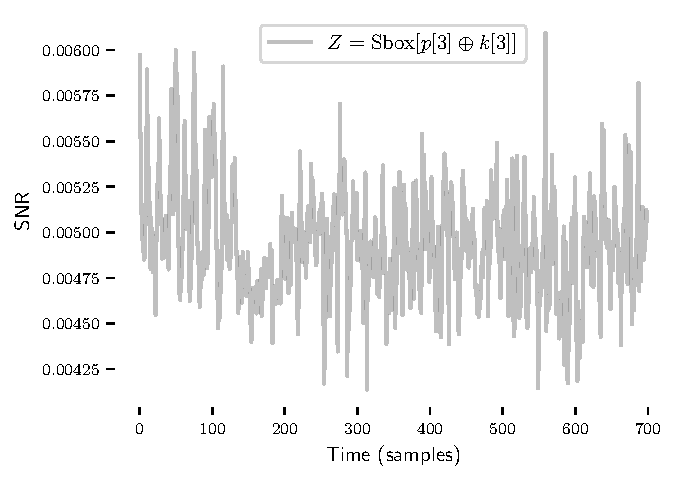
\includegraphics[width=\textwidth]{ASCAD/snr_raw}
        \caption{Characterization without knowledge of the secret shares.}
        \label{fig:charac_ascad_mask}
    \end{subfigure}
    \begin{subfigure}{0.49 \textwidth}
        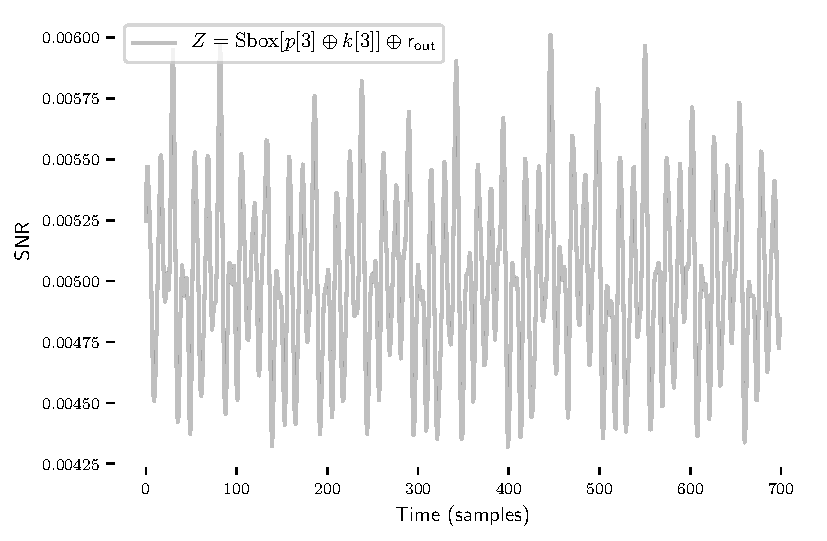
\includegraphics[width=\textwidth]{ASCAD/snr_desync50}
        \caption{Characterization on randomly shifted traces (\(T=50\)).}
        \label{fig:charac_ascad_shift}
    \end{subfigure}
    \caption{Effect of the counter-measures to the characterization on the \gls{ascad} dataset.}
    \label{fig:charac_ascad_cm}
\end{figure}

\subsection{Random Delay Dataset (AES-RD)}
\label{sec:aesrd}
The \gls{aesrd} dataset has been released, following the works of Coron \etal{} on the insertion of random delays in the implementation of a software AES, as a way to implement the dummy operation insertion~\cite{coron_random_2009,coron_random_2010}.
In a nutshell, it consists in drawing -- thanks to the \gls{prng} -- a random number of cycles during which a loop will iterate.

\paragraph{The Target.}
The target smart-card is an 8-bit \textsf{Atmel AVR} micro-controller, protected by a random delay counter-measure, which has an effect on the misalignment of the traces, making some attacks such as with \glspl{gta} much harder.
The targeted variable is the output of the first \(\Sbox\).
The dataset is publicly available at \url{https://github.com/ikizhvatov/randomdelays-traces}.
\(50,000\) traces of \(\traceLength = 3,500\) time samples each are provided, denoting the power consumption of the target.
These power traces have been previously compressed by selecting 1 sample (peak) from each \gls{cpu} clock cycle.
At least the first (non-dummy) \gls{aes} round is covered.
In this thesis, we split the dataset into \(\numTracesProf = 40,000\) profiling traces and \(\numTracesVal = 10,000\) validation traces.

\paragraph{Quick Analysis of the Traces.}
We provide in \autoref{fig:snr_aes_rd} an example of trace from the dataset (top), along with a characterization with \gls{snr} over the whole dataset (bottom).
\begin{figure}
    \centering
    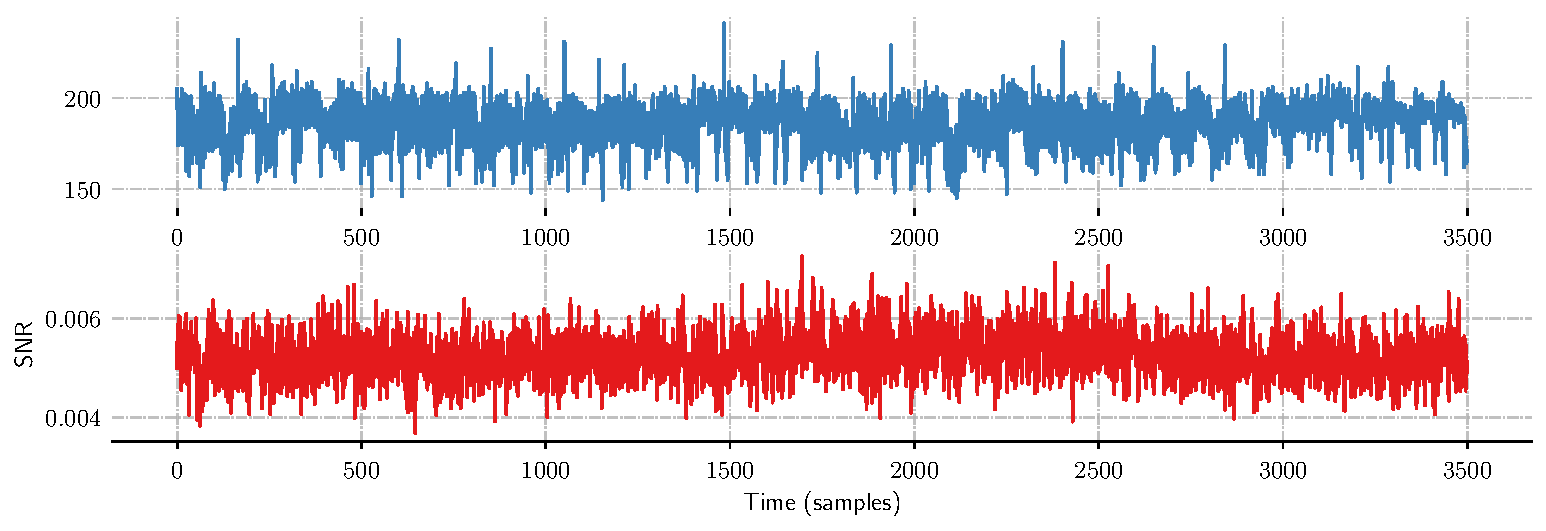
\includegraphics[width=\textwidth]{AES-RD/snr}
    \caption{Top: An example of a trace from the \gls{aesrd} dataset.
    Bottom: the \gls{snr} computed over the whole dataset.}
    \label{fig:snr_aes_rd}
\end{figure}
As expected, due to the misalignment effect of the random delay counter-measure, no peak denoting a leakage is emphasized.
This confirms that either a pre-processing phase including re-alignment or the use of a misalignment-resilient methods is necessary to deal with those traces.

\subsection{AES on FPGA (AES-HD)}
\label{sec:aeshd}
The \gls{aeshd} dataset has been released by Picek \etal{} at \textsc{Ches} 2019~\cite{picek_curse_2019}, in order to introduce a dataset of \gls{sca} traces targeting a hardware implementation whereas the majority of the public datasets are focused on software implementations.
Moreover, this dataset is an example of use-case where the targeted sensitive variable comes from the last round of the \gls{aes} encryption.

\paragraph{The Target.}
We recall hereafter the description provided by Picek \etal{} in their paper.
This is an ``unprotected implementation of \gls{aes}, written in \gls{vhdl} in a round based architecture taking 11 clock cycles for each encryption.
The design was implemented on a \textsf{Xilinx Virtex-5} \gls{fpga} of a \textsf{SASEBO GII} evaluation board. 
Side-channel traces were measured using a high sensitivity near-field \gls{em} probe,
placed over a decoupling capacitor on the power line.''
The dataset is publicly available at \url{https://github.com/AESHD/AES_HD_Dataset}.

The authors recommend to use an intermediate leakage model \(\varphi\) corresponding to the Hamming distance between the targeted byte of the state before applying the \(\Sbox\) of the last round, and the final ciphertext byte.
In the following of this thesis, we will rather target the input of the last \(\ark\), without considering any prior leakage model.

\paragraph{Quick Analysis of the Traces.}
\autoref{fig:snr_aes_hd} provides a brief insight of the traces.
\begin{figure}
    \centering
    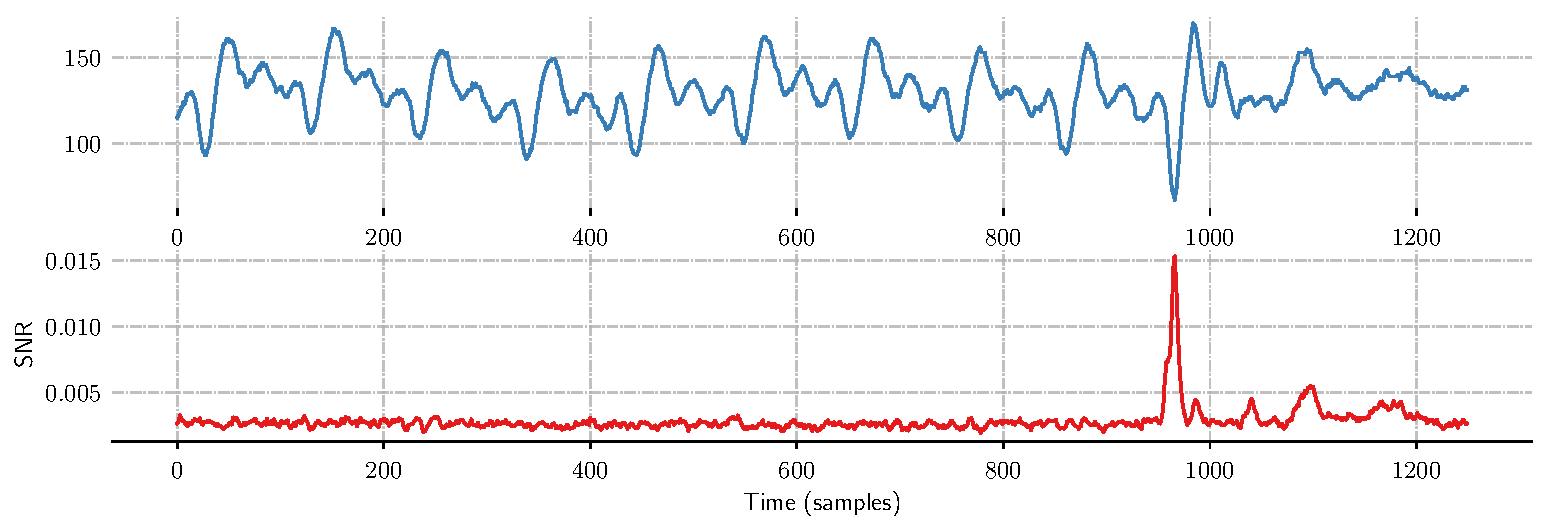
\includegraphics[width=\textwidth]{AES-HD/snr}
    \caption{Top: one trace of the \gls{aeshd} dataset.
    Bottom: The SNR computed over the whole dataset.}
    \label{fig:snr_aes_hd}
\end{figure}
One can guess 10 similar patterns corresponding to the 10 rounds of \gls{aes}.
The peak of \gls{snr} appears on the last pattern, confirming that the targeted sensitive variable is an intermediate computation of the last round.
Although the peak is clearly distinguishable, one may remark that the peak is at approximately \(0.15\), which is lower than the preceding \glspl{snr} observed in \autoref{fig:snr_cw} and \autoref{fig:charac_ascad_snr}.
This is expected since hardware implementations are known to usually leak less information.


\subsection{Polymorphism Dataset}
\label{sec:claps_ds}
In \autoref{chap:dl_sca_practice}, we will present the investigations conducted on the security of the code polymorphism counter-measure proposed by Belleville \etal{}~\cite{belleville_automated_2019}.
To this end, we conducted an acquisition campaign of \gls{sca} traces over two out of the 15 implementations used in their benchmarks, namely the \aeshuitbit{} and the \mbedTLS{} that we briefly describe hereafter, along with the details of the experimental setup and a preliminary analysis.

\paragraph{The \mbedTLS{} Implementation.}
This \(32\)-bit implementation of \gls{aes} from the \textsf{ARM} library~\cite{mbed_tls_code} follows the so-called \emph{T-table} technique~\cite{AES_rijndael_2002}: the \(16\)-byte state of \gls{aes} is encoded into four \verb+uint32_t+ variables, each representing a column of the state.
Each round of the \gls{aes} is done by applying four different constant \glspl{lut} stored in flash memory.

\paragraph{The \aeshuitbit{} Implementation.}
This is a simple software unprotected implementation of \gls{aes} written in \textsf{C}, and manipulating only variables of type \verb+uint8_t+, similar to \cite{SmallportableAES1282020}.
The \(\sub\) operation is computed byte-wise thanks to a \gls{lut}, stored in \gls{ram}.
This reduces information leakage on memory accesses, compared to the use of the same \gls{lut} stored in flash memory.

\paragraph{Target Device.}
We ran the different AES implementations on an \textsf{STM32 NUCLEO F303} board, embedding an \textsf{ARM Cortex-M4} \(32\)-bit core~\cite{STMicroelectronicsNUCLEOF303RE}.
This device does not provide any hardware security mechanisms against side-channel attacks.
This core originally operates at \(72\)~MHz, but the core frequency was reduced to \(8\)~MHz for the purpose of side-channel measurements.
The target is similar to the one used by Belleville \etal{}~\cite{belleville_automated_2019}, who considered a \textsf{Cortex-M3} core running at \(24\)~MHz.
These two micro-controllers have an in-order pipeline architecture, but with a different pipeline organization.
Thus, we cannot expect those two platforms to exhibit the same side-channel characteristics.
However, our experience indicates that these two experimental setups would lead to similar conclusions regarding the attacker models considered in our study.
Similar findings on similar targets have also been reported by Heuser \etal{}~\cite{heuser_physical_2020}.
Therefore, we assume that the differences of side-channel characteristics between our targets and the Belleville \etal{}'s ones should not induce major differences in the results of such side-channel analysis.

\paragraph{Configuration of the Code Polymorphism Counter-Measure.}
For each evaluated implementation, the code polymorphism counter-measure is applied with a level corresponding to the configuration ``\textsf{high}'' described by Belleville \etal{}~\cite{belleville_automated_2019}: all the polymorphic code transformations  are activated, the number of inserted noise instructions follows a probability distribution based on a truncated geometric law.
The dynamic noise is activated and \glspl{sgpc} produce a new polymorphic instance of the protected code for \emph{each} execution (\ie{}, the regeneration period is set to 1).

\paragraph{Acquisition Setup.}
\label{sec:setup}
We measured \gls{sca} traces corresponding to \gls{em} emanations with an \gls{em} probe \textsf{RF-B 0.3-3} from Langer, equipped with a pre-amplifier, and a \textsf{Rohde \& Schwarz RTO} \(2044\) oscilloscope with a \(4\) GHz bandwidth and a vertical resolution of \(8\)~bits.
We set the sampling rate to \(200\)~MS/sec., with the acquisition mode ``\emph{peak-detect}' which collects the minimum and the maximum voltage values over each sampling period.
We first verify that our acquisition setup is properly set.
This is done by acquiring several traces where the code polymorphism is de-activated.
Thus, we can verify that those traces are synchronized.
Then, computing the T-test (\cf{} \autoref{sec:PoIs}) enables to quickly\footnote{\ie{}, faster than with a \gls{snr} computation.} assess whether the probe is correctly positioned and the sampling rate is high enough.
Then, after re-activating the code polymorphism, \(100,000\) profiling traces are acquired for each target implementation.
Each acquisition campaign lasts about \(12\) hours.

\paragraph{Preliminary Analysis of the Traces.}
\label{sec:visual_inspect}
We detail hereafter a preliminary analysis of the acquired traces.
The aim is to restrict as much as possible the target region acquired to a window covering the entire first \gls{aes} round.
Therefore there would not be any loss of informative leakage about the sensitive intermediate variable targeted in those experiments.
In addition to that, a uni-variate leakage assessment, by computing the \gls{snr}, is provided hereafter in order to verify that there is no trivial leakage.

\subparagraph{\mbedTLS{}.}
We ran some preliminary acquisitions on \(10^7\) samples, in order to visualize all the execution.
We could clearly distinguish the \gls{aes} execution with sparse \gls{em} peaks, from the call to the \gls{sgpc} with more frequent \gls{em} peaks.
This enabled to focus on the first \(10^6\) samples of the traces corresponding to the \gls{aes} execution.

Actually, the traces restricted to the \gls{aes} execution seem to remain globally the same between each other, up to local elastic deformations along the time axis.
This is in line with the expected effect of code polymorphism, since it involves transformations at the machine code level.
Likewise, \(10\) patterns could be distinguished on each trace, which were clues to expect that it would correspond to the \(10\) rounds of \gls{aes}. 
That is how we could restrict again our target window to the first round, up to comfortable margins because of the misalignment effect of code polymorphism.
This represents \(80,000\) samples.
An illustration of two traces restricted to the first round is given by \autoref{fig:observations_v1} (top).%
\footnote{Here the first \(20\ \mu\)s of both traces correspond to a non-critical part of the implementation, probably due to the \gls{os} of the chip.
Hence the apparent synchronization here.}

\begin{figure}[t]
	\centering
	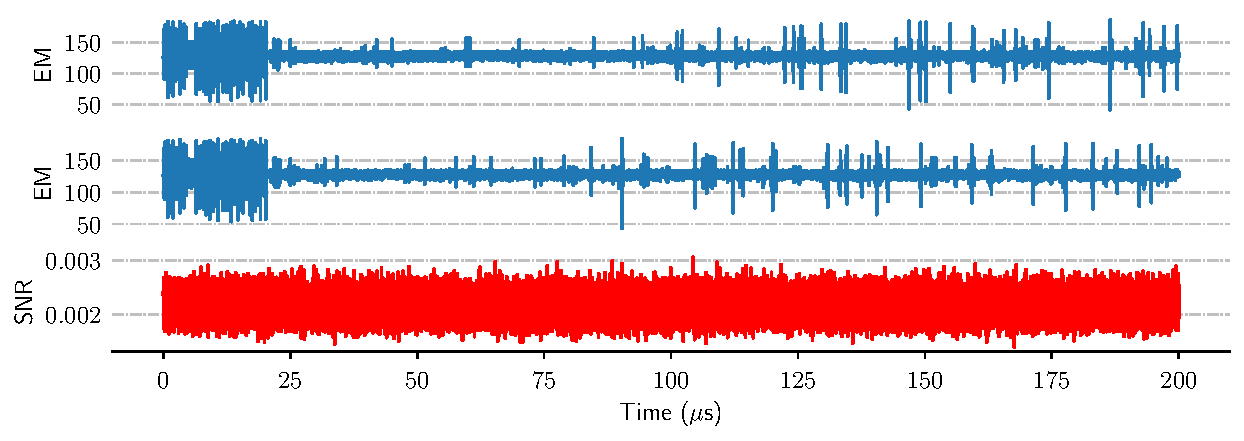
\includegraphics[width=\textwidth]{CLAPS/v1/snr_raw}
	\caption{Acquisitions on the \mbedTLS{} implementation.
	Top: two traces containing the first AES round.
	Bottom: SNR computed on the \(100,000\) profiling traces.}
	\label{fig:observations_v1}
\end{figure}

% SNR computation
The \gls{snr} denoting here the potential uni-variate leakage of the first output byte of the \sub{} operation is computed based on the \(100,000\) acquired profiling traces, and is plotted in \autoref{fig:observations_v1} (bottom).
No distinguishing peak can be observed, which confirms the soundness of code polymorphism against attacks requiring the \glspl{poi} of the raw traces to be aligned with each other, \eg{}, the \gls{cpa} or the \gls{gta}.

% Realignment
However, we observe in each trace approximately 16 \gls{em} peaks corresponding to the number of memory accesses to the \glspl{lut} per encryption round.
These memory accesses are known to carry sensitive information.
This suggests that a trace re-alignment on \gls{em} peaks might be relevant to successfully achieve such attacks.%
\footnote{
    A re-alignment process is proposed in \autoref{sec:method}.
}

\subparagraph{\aeshuitbit{}.}
We proceed in the same way for the evaluation of \aeshuitbit{} implementation.
As with the \mbedTLS{} traces, we could identify \(10\) successive patterns likely to correspond to the \(10\) \gls{aes} rounds.
Therefore we reduce the target window at the oscilloscope to the first \gls{aes} round, which represents \(160,000\)-dimensional traces plotted in \autoref{fig:observations_v2} (top).
\begin{figure}[t]
	\centering
	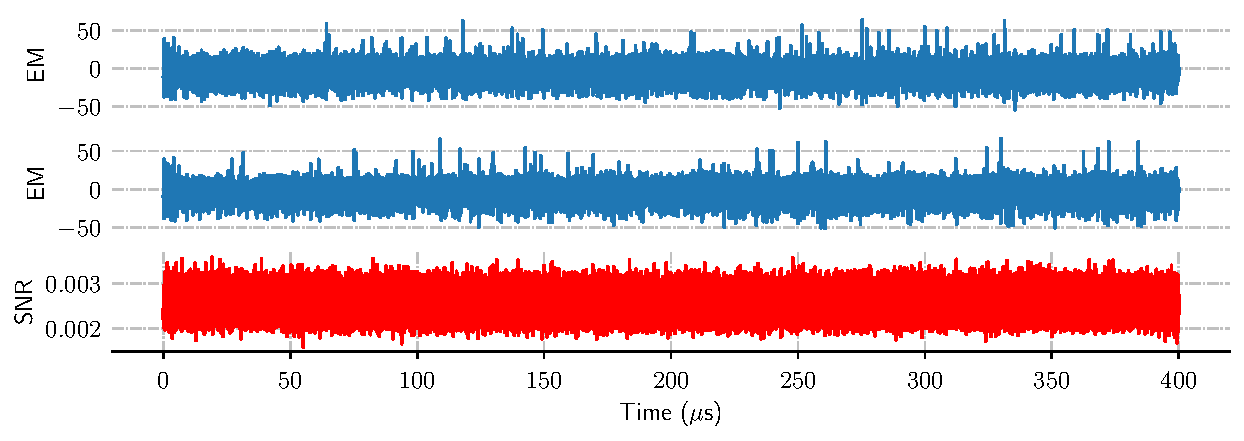
\includegraphics[width=\textwidth]{CLAPS/v2/snr_raw}
	\caption{Acquisitions on the \aeshuitbit{} implementation.
	Top: two traces containing the first \gls{aes} round.
	Bottom: \gls{snr} computed on the \(100,000\) profiling traces.}
	\label{fig:observations_v2}
\end{figure}
This growth in the size of the traces is expected, since the naive \aeshuitbit{} implementation is not optimized to be fast, contrary to the \mbedTLS{} one.

Yet, here the peaks are hardly distinguishable from the level of noise.
This is expected, due to the \glspl{lut} being moved from the flash memory to the \gls{ram}.
As a consequence, the memory accesses are less remarkable.
That is why a trace re-alignment does not seem relevant here.

Finally, \autoref{fig:observations_v2} (bottom) shows the SNR on the raw traces, ensuring once again that no trivial leakage can be exploited to recover the secret key.